%% ------------------------------------------------------------------------- %%
\chapter{Introduction}
\label{cap:Introduction}

Hash functions and hash tables are among the most classic topics within computer science, yet is still one of the topics with most debate about what is state of the art. While the hash table was invented in 1953, widely discussed by Donald Knuth in his famous book The Art of Computer Programming (Vol.3, Chapter 6.4), there are still many tweaks that can be made to boost its performance for specific use cases. One great example is F14, an open-source memory efficient hash table by Facebook \footnote{F14 is open sourced: \url{https://engineering.fb.com/developer-tools/f14/}}.

An example of lack of consensus in this area are the different hash functions and hash table implementations in different languages. There is no clear consensus on how to decide the size of a hash table, what are the tradeoffs of the collision-resolution algorithms or even what defines a good hash function. Hopefully, we got years of research on the topic to study and present a view on the subject, and that is what I am presenting thoughout this undegraduate thesis.

During this introduction I give a brief idea of what are hash functions, hash tables and why they are interesting. This will also give you a grasp of what you can expect to read about in each chapter.

\section{Hash Functions}

Outside computer science, the word \textit{``hash''} in the english language means to ``chop'' or to ``mix'' something. This meaning is entirely related to what hash functions are supposed to do. hash functions are functions that are used to map data of an arbitrary size to data of a fized size \cite{HashFuncWiki}.

They have wide applications in computer science, being used in information and data scurity, compilers, distributed systems and hardcore algorithms. During this thesis I first define and explain the basics of a hash function, then I give an intiution in some metrics of what is a good hash function, as discussed in the famous \textit{``Red Dragon Book''} \cite{DragonBook} along with some reproduction of known results in the area.

The value extracted from the hash function for an object is usually called \textit{Hash Value}. The hash value is usually, but not necessarily, smaller than the object that generated it. For example, we can have a hash function that takes Gigabytes or Terabytes files and return an 8 bytes hash value.

\begin{figure}[h!]
  \centering
  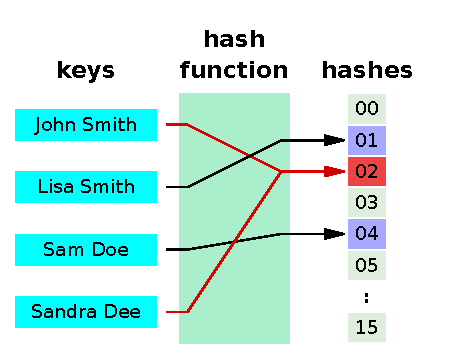
\includegraphics[width=12cm]{figuras/hash-function.pdf}
  \caption{Example of a hash function from string to 4 bit integer. }
\end{figure}

\section{Hash Tables}

Hash tables or hash maps is one of the most used applications of hash functions. It is actually so used in computer science that is almost impossible to talk about one without mentioning the other. This data structure consists in associating a \textit{key} to a \textit{value} in a table. That is, given a \textit{key}, it can retrieve the correct \textit{value} for it.

This data structure is usually considered very useful among software engineers and computer scientists, although it usually has a linear worst case cost for retrieving, inserting and deleting a key a value pair. That is because it has a constant average and amortized cost for those operations.

Moreover, when talking about hash tables we have the problem of key collision, that is when two keys maps to the same hash value. To solve that problem, we have several techniques that envolves different tradeoffs. Those techniques are usually divided into two main categories, open addressing and separate chaining. Other problem to consider regarding this data structure is when to resize the hash table, to minimize the chance of collision and the use o memory.

It is also important to notice that hash tables have applications in different areas of computer science also, like compilers, caches and database indexing.


\begin{figure}[h!]
  \centering
  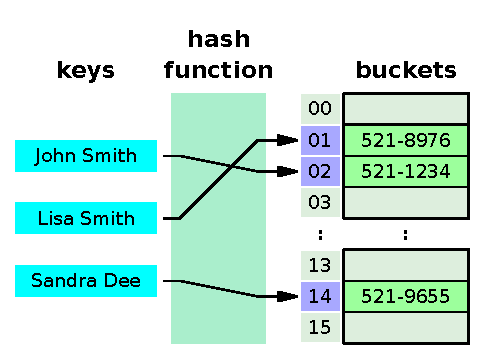
\includegraphics[width=12cm]{figuras/hash-table.pdf}
  \caption{Example of a hash table from string to string, more specifically name to number}
\end{figure}

\section{Applications}

Hash functions and hash tables have a great number of applications in computer science. During this last section I focus on applications of hash functions in algorithms, but citing superficially applications in other areas (like criptography, data deduplication and caching).

Among the applications that I explain in this section there is a focus in two applications: Rabin-Karp string matching algorithm and hashing of a rooted tree for isomorphism checking. Rabin-karp string matching algorithm is one of the main application of a technique called rolling hashing. Hahsing of rooted tree for isomorphism checking is an interesting application sometimes used in competitive programming.

To motivate the start of this thesis I will start using hash tables to solve a very simple, yet famous, problem called 3-sum.

\subsection{3-sum problem}

The problem is stated as following:

\textit{Make a function that given an array of integer numbers and an integer S, it returns if there are any 3 different elements in this array that its sum equals S. Assume that there are no three different elements in the array that overflow a 32-bit integer when summed together.}

This a very interesting problem that has many different solutions. To start I will show and explain to you the brute force solution: \\
\\
\bigskip

\begin{lstlisting}
bool threeSumWithoutHashTable(vector<int> v, int S) {
   for (int i = 0; i < v.size(); i++) {
      for (int j = i + 1; j < v.size(); j++) {
         for (int k = j + 1; k < v.size(); k++) {
            if (v[i] + v[j] + v[k] == S) return true;
         }
      }
   }
   return false;
}
\end{lstlisting}

\medskip

The above solution solves the problem in \( O(n^3) \) time complexity and \( O(1) \) memory complexity, being \( n \) the size of the array. It don't allocate any memory but checks every triple to find if one satisfy the condition. The question is, can we do better in time complexity using hash tables? The answer is yes:

\medskip

\begin{lstlisting}
bool threeSumWithHashTable(vector<int> v, int S) {
   unordered_map<int, int> hashTable; 
   for (int i = 0; i < v.size(); i++) {
      hashTable[v[i]]++;
   }
   for (int i = 0; i < v.size(); i++) {
      for (int j = i + 1; j < v.size(); j++) {
         hashTable[v[i]]--;
         hashTable[v[j]]--;         
         if (hashTable.find(S - v[i] - v[j]) != hashTable.end() &&
             hashTable[S - v[i] - v[j]] > 0) return true;
         hashTable[v[i]]++;
         hashTable[v[j]]++;
      }
   }
   return false;
}
\end{lstlisting}

\medskip

The above solution solves the problem in \( \Theta(n^2) \), time complexity (average and amortized) and \( O(n) \) memory complexity. Although the worst case scenario is \( O(n^3) \) and it uses more memory, this solution is way faster in practice for large input cases. To showcase this I made simmulations with the codes shown (that can be found in bibliography), the results are: \\

\bigskip

\begin{tabular}{|l|l|l|l|}
  \hline
  ArraySize & Time Without Hash Table & Time with Hash Table & Increase in Performance \\
  \hline
  128       & 4.231ms                 & 6.494ms              & -53.4\%                  \\
  \hline
  256       & 34.223ms                & 26.665ms             & 22.0\%                   \\
  \hline
  512       & 267.499ms               & 99.130ms             & 62.9\%                   \\
  \hline
  1024      & 1742.688ms              & 302.453ms            & 82.6\%                   \\
  \hline
  2048      & 7345.126ms              & 683.197ms            & 90.6\%                   \\
  \hline
  4096      & 25029.888ms             & 761.363ms            & 96.9\%                   \\
  \hline
\end{tabular}

\bigskip

As we can see for the table above, the three sum solution using hash table quickly surpasses the brute force implementation. As we will see later, hash tables (or \textit{unordered\_map}) are not the fastest hash tables possible \cite{UnorderedMapDiscussion}. That means we can have an even greater performance than what is shown now.  